\documentclass[letterpaper]{article}
\usepackage[margin=1in]{geometry}
\usepackage[shortlabels]{enumitem}
\usepackage{amsmath,amssymb,amsthm,dsfont}
\usepackage{setspace,parskip,multicol,titling}
\usepackage{graphicx}

\newcommand{\R}{\mathds{R}}
\newcommand{\Z}{\mathds{Z}}
\newcommand{\Q}{\mathds{Q}}
\newcommand{\C}{\mathds{C}}

\newcommand{\nope}{\textbf{DO THIS}}
\newcommand{\group}[1]{\langle \, #1 \, \rangle}
\renewcommand{\b}[1]{\textbf{#1}}

\setlength{\droptitle}{-1cm}
\setlength\parindent{0pt}
\setlength\parskip{8pt}
\setstretch{1.60}
\setlist{leftmargin=0.25in}

\title{CSC 258 Project: Elixir Game}
\author{Brandon Willett}

\begin{document}

	\maketitle

	\section{Introduction}

	I don't really play video games anymore, but back when I was in high school, it was the main way my friends and I would pass the time after classes let out. The one we played the most was called World of Warcraft, where you play as an Elf or an Orc (or something), and you'd complete quests to level up and get better gear for your character. Doing quests was fun, but my favorite part of the game came only at the end, when you reached the maximum level -- then, you could start doing ``raids'', where groups of up to 40 players would team up and attempt to defeat massive boss enemies together. These bosses had abilities that could wipe out your entire team in one shot, so not only were individual players' skill and reaction times important, but also the overall group's composition: if you had too many high-damage-output members, the whole team would die before the boss could be killed, since those types tend to be fragile. Or, if you had too many healing characters, the entire raid might never end, since you might never kill a boss at all!

	These exercises in teamwork and perseverance were a lot of fun for me at the time, and in fact they represent a pretty complicated distributed system. There are 40 players all rapidly sending commands to a central location which affect the boss's health and condition, and each of these players need there to be almost zero latency and perfect delivery of their messages, which -- when the ``central location'' is made up of many machines which might fail -- is hard to accomplish; the continuous synchronization of these messages is a challenge. In addition, each client needs to not only send ``damage the boss'' messages to the central location, but also to listen for ``you've been healed'' messages back from others. This sort of player-count-agnostic system is required, since at any one time there might be 4 or 40 players sending messages at once, and this too presents an interesting issue.

	Thus, we reach the idea of my project, which is to implement a simplified version of this game as a command line app in Elixir. At any time, a client can ``join the fight'' either as a healer or a damage character. Then, they'll have a set of commands they can send to the remote server, like querying the boss's current health or executing a move to heal a friend whose character is in danger of dying. While Elixir as a language (being focused on many independent message-passing processes) is a great fit for the task, it also represents the ``hard part'' of this project, since up until this point I'd never used the language before, and this style of programming requires a very different mindset than usual.

	\section{Outline}

	One reason that Elixir was a good choice to model this task is that its OTP (Open Telecom Platform, inherited from Erlang) framework was designed to make this exact type of program easy to write. The general model relies on a large number of cheap independent processes, which can be distributed just as easily among the system threads of one computer or the machines of a server farm. Each process has its own state that it manages, and they can affect each others' states only via message passing, which also scales in a simple and easy way. The only trouble is, with that many concurrent processes all running at once, the chance of a process failing is high, and in normal circumstances, one important process failing brings down the whole system. To combat this, the OTP model makes extensive use of ``Supervisors'' -- processes whose only job is to monitor other processes, and cleanly restart them if they fail. In this way, a well-designed Elixir application can have any number of failing worker processes, and a user would never notice.

	In our Elixir game, most of these worker processes are set up to be players; whenever a player logs into they game, they get their own worker to monitor their health and send/receive messages for them (\texttt{PlayerAgent.ex}). This choice was made to simulate a larger-scale program with actual work to do (beyond just incrementing a player's health points), where the workers would perform tasks that had an actual chance of failing. Thus, we make sure that all players are supervised by a supervisor (\texttt{PlayerSupervisor.ex}), making the system quite fault-tolerant. In addition, the boss also has its own resilient process (in \texttt{BossAgent.ex}), with methods for healing itself and a ``stomp'' which damages all players, and its own supervisor for restarting if it fails (\texttt{BossSupervisor.ex}).

	The last important component of the game, working a bit more behind the scenes, is the player process registry. We'd like to be able to heal our teammates by name, but in the case that their process fails, they'll be put back up and running with a new and different process ID, so a straight mapping can't work. Instead, we use a hand-built process registry -- whenever a new player process is started (or restarted), right after getting its last known health from a data store (in this case cache), it registers its name to its PID in the registry (\texttt{PlayerRegistry.ex}). In this way, even in the presence of failures, we have an up-to-date (and also supervised) mapping from player names to their PIDs, so we never send a message to a dead process. I built my own, but this pattern is so common with Elixir applications that it has a built-in process registry!

	\begin{figure}[ht]
		\centering
		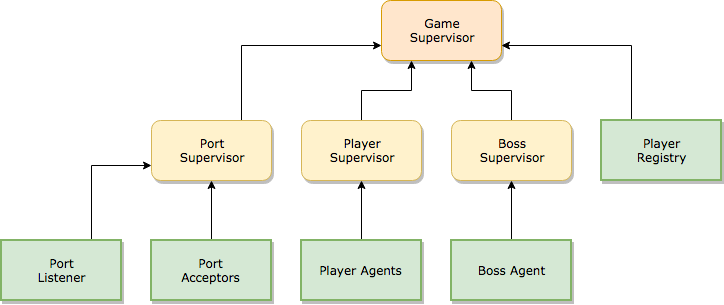
\includegraphics[width=0.8\textwidth]{Diagram}
		\\[1.5em]
		\caption{A general overview of the Elixir Game's supervision tree}
		\label{fig:mesh1}
		\vspace*{12pt}
	\end{figure}

	\section{Implementation Details}

	To show the detailed running of the program, we can walk through an example sequence of events.

	First, on startup, the overall supervisor (highest in the supervision tree) starts the supervisors for Players, the Boss, the Registry, and the Ports (see Figure 1). Then, the Boss supervisor begins a Boss process, which automatically registers itself as "Charlie" (the boss's name) under the Registry and begins to stomp, using the registry's \texttt{dispatch} function to send a damaging message to all players in the registry. In addition, the Port supervisor begins to listen on localhost, port 6666. 

	When a player connects, the Port Supervisor spawns a new Task process to serve the user, ensuring it can continue to listen for other players and not be busy dealing with \texttt{telnet} messages. Then, methods in \texttt{Input.ex} help manage and direct what to do with a user's input: when they type \texttt{signup Brandon}, for example, it sends the (dynamic) Player Supervisor a message to spawn and register a new player named Brandon. Then, all subsequent messages of Brandon are sent through the Registry to find the correct PID, and handled by the backend GenServer instance of each player process.

	Finally, when a player process (or literally any other process in the application, even a supervisor) dies, the Player Supervisor will restart a new process for it, which will immediately register the name under a new PID with the Registry, and also check the cache (or some generic data store) to find the last-known health for that player. That way, even if a process dies in the middle of handling a message, it'll be started up again quickly, affecting no other players, and only that single message will be lost in the process.

	\begin{figure}[ht]
		\centering
		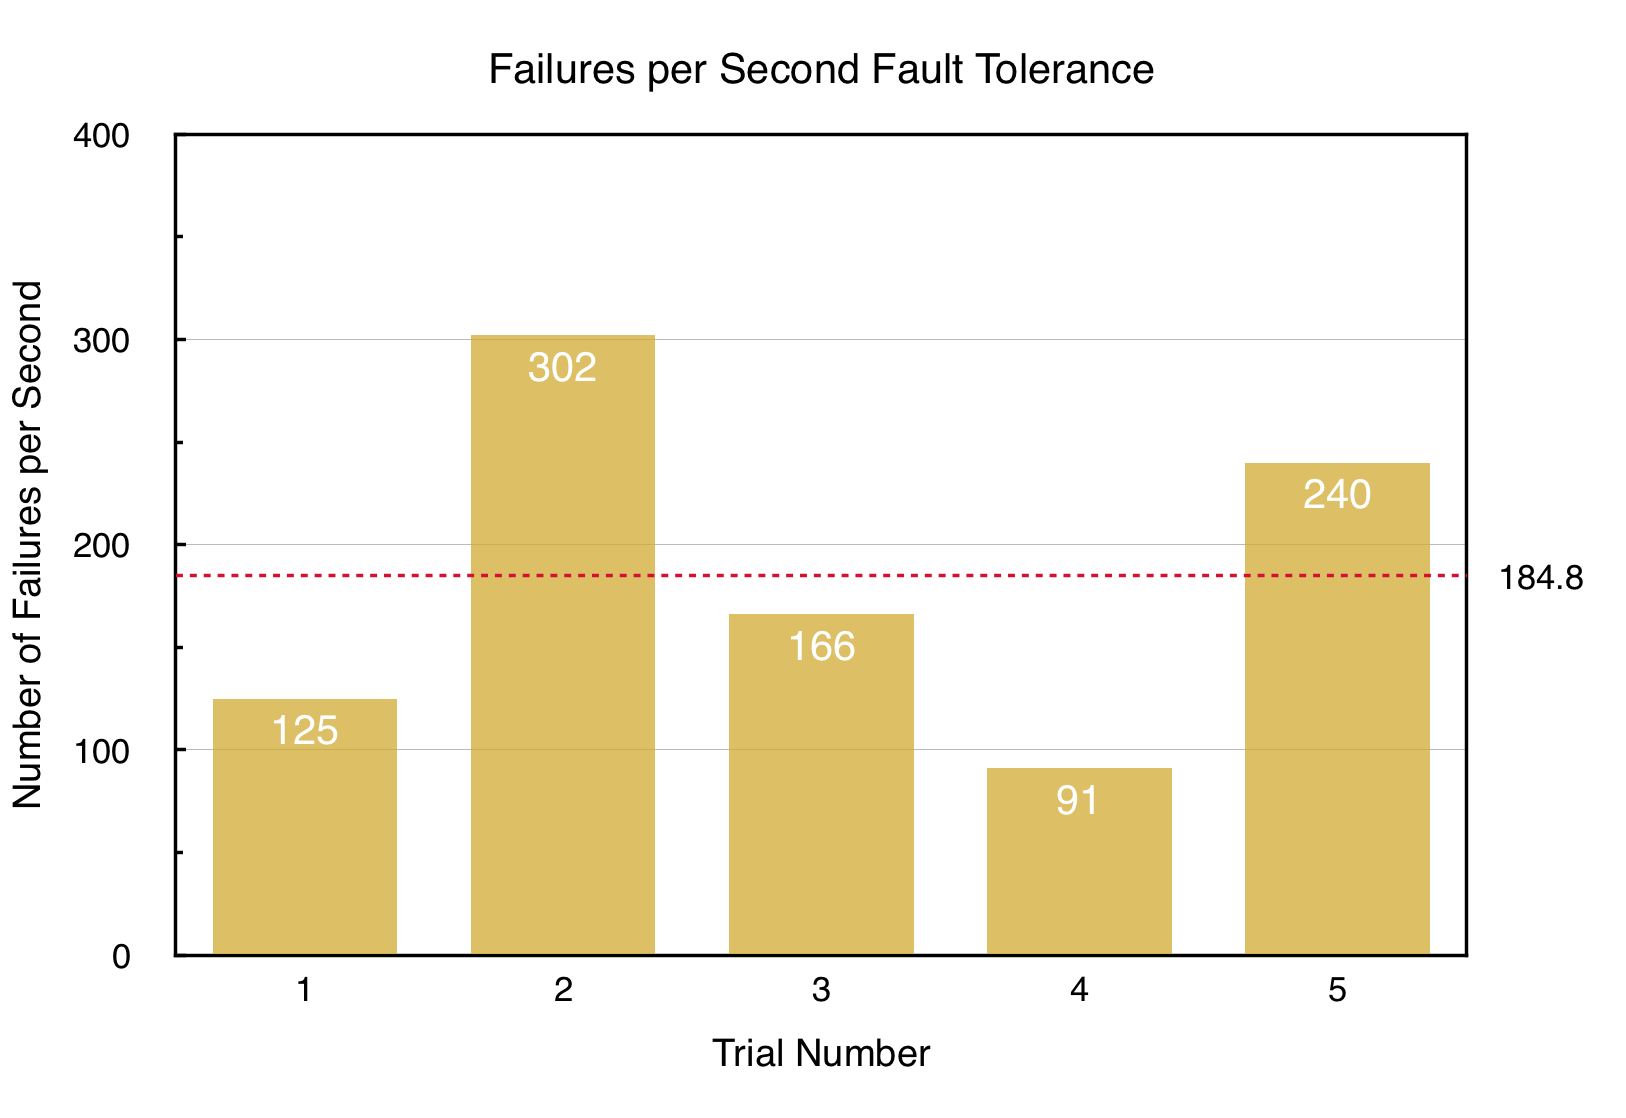
\includegraphics[width=0.8\textwidth]{failures}
		\caption{A general overview of the Elixir Game's supervision tree}
		\label{fig:mesh2}
		\vspace*{12pt}
	\end{figure}

	\section{Experiments}

	\textbf{Note: This project wasn't based on parallelizing a long-running serial task, so there can't much in the way of raw data or experimental comparisons.}

	In order to try and make up for this, I tried to implement what I think is the next-best thing that does apply to this project, which is a pretty extensive suite of unit tests. As documented in the README, those can be found in the ``test'' folder and run with \texttt{mix test}. They run from simple things, like starting up a new player and making sure the boss can be damaged, to the most important parts of the project, like killing a player's process and then making sure it's automatically restarted with their current health being consistent with what it was before the process died.

	In addition, in order to highlight how quickly processes can be restarted on the BEAM VM (which is the underlying virtual machine of all Erlang and thus Elixir programs), I attempted to run some tests to determine how many times a player's governing process could be forcefully killed (per second) while still responding to commands from an outside source. As we see in Figure 2, it's a pretty large number, at an average of over 100 deaths per second. This is another testament to the fault-tolerance of a system built in Elixir with the OTP framework -- even if thousands of processes died at once, their supervisors would have them all up and running again in a fraction of a second, which is vital for this kind of system.

	\section{Citations}

	\begin{itemize}

		\item Introduction to Mix and OTP frameworks\\
		\verb|https://elixir-lang.org/getting-started/mix-otp/introduction-to-mix.html|

		\item ``Learn You Some Erlang for Great Good'' Guide for Process Management\\
		\verb|http://learnyousomeerlang.com/content|

		\item Documentation for Elixir and Mix and IEX unit tests (great documentation)\\
		\verb|https://hexdocs.pm/elixir/Kernel.html|

		\item Process registry in Elixir: A practical example\\
		\verb|https://m.alphasights.com/process-registry-in-elixir-a-practical-example-4500ee7c0dcc|

	\end{itemize}

\end{document}








